\begin{figure}[htb]\centering
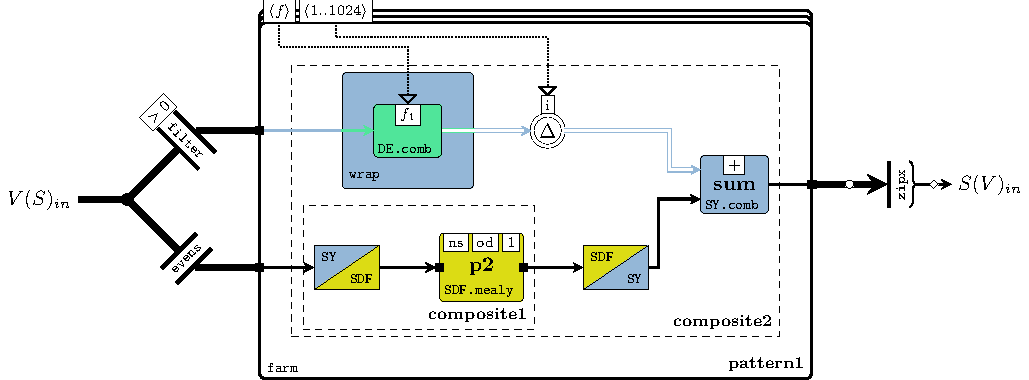
\includegraphics[width=\textwidth]{figs/example-forsyde-tikz}
\end{figure}
\lstinputlisting{figs/example-forsyde-tikz.tex}

\section{The \texttt{forsyde-tikz} package}


This library is used to draw systems modeled as process networks with \ForSyDe, similar to the one on the previous page. A \ForSyDe process network is drawn like any other \textsc{TikZ} figure, inside a \texttt{tikzpicture} environment. The \texttt{options} provided are key variables defined by the \texttt{tikz} package. \bookmark{environment}

\begin{verbatim}
	\begin{tikzpicture}[options]
          content...
	\end{tikzpicture}
\end{verbatim}

Apart from the standard keys, \texttt{forsyde-tikz} provides the following variables:\bookmark{environment variables}
\begin{optionslist}
\item \texttt{no moc color} : disables process coloring according to their MoC.
\item \texttt{no moc label} : disables process labeling according to their MoC.
\item \texttt{label style=} : font style for the process type labels. Default is \texttt{\char`\\ textbf}.
\item \texttt{type style=} : font style for the process name labels. Default is \texttt{\char`\\ scriptsize\char`\\textit}.
\item \texttt{function style=} : font style for the functions. Default is \texttt{\char`\\ scriptsize}.
\end{optionslist}

\subsection{Main nodes}

Using \texttt{forsyde-tikz}, process networks are drawn using a combination of commands and style options for customizing shapes. 

\subsubsection{Draw commands}
\label{sec:draw-commands}

Inside the \texttt{tikzpicture} environment, one can use a set of draw commands which are used as templates for placing shapes and information provided as arguments. In the following listing, the \opt{gray}\man{} arguments are optional while the \man{black} ones are mandatory. 
The library also provide as set of helper styles for setting several options at once, presented in \ref{sec:helper-options}.\\

\begin{figure}[htb]\centering
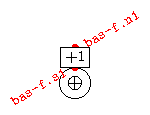
\includegraphics{figs/example-node-basic}
\lstinputlisting[linerange={5-5}]{figs/example-node-basic.tex}
\caption{The \texttt{\char`\\basic} draw command. The red dots are custom anchors, accessed with \texttt{[name]-f.[anchor]}.}
\end{figure}
\hspace{1pt}\bookmark{\char`\\basic\opt{[options]}\opt{(name)}\opt{<position>}\man{\{label\}};}

\noindent The basic node is the simplest depiction of a function (e.g., process, atom) with maximum one argument. It is the most lightweight graphical primitive, and does not contain port anchors. It can be customized with the following keys (check \ref{sec:helper-options} for composite options):

\begin{optionslist}
\item \texttt{shape=} any \texttt{TikZ} style option for the node shape. Check section \ref{sec:provided-shapes} for a list of library-provided shapes. Default is \texttt{rectangle}.
\item \texttt{nf=[0..1]} the number of passed functions. Default is \texttt{0}. If \texttt{nf>1} then \texttt{nf=1}.
\item \texttt{f1=} function label. Appears as a box above the main shape in case \texttt{nf > 0}. Default is $f_1$.
\item \texttt{anchor=[anchor]} center point for shape. Default is \texttt{center}.
\item \texttt{xshift=[distance]} shift position in X direction. Default is \texttt{0pt}.
\item \texttt{yshift=[distance]} shift position in Y direction. Default is \texttt{0pt}.
\end{optionslist}


\begin{figure}[htb]\centering
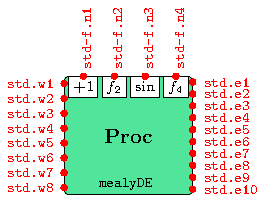
\includegraphics{figs/example-node-standard}
\lstinputlisting[linerange={5-5}]{figs/example-node-standard.tex}
\caption{The \texttt{\char`\\standard} draw command. The function anchors are accessed with \texttt{[name]-f.[anchor]} and the port anchors are accessed with \texttt{[name].[anchor]}}
\end{figure}
\hspace{1pt}\bookmark{\char`\\standard\opt{[options]}\opt{(name)}\opt{<position>}\man{\{label\}};}

\noindent The standard node is a more complex depiction of a ForSyDe block. It contains anchors for each port, shows a label and the constructor name, and its field is colored according to a MoC (if this is the case). It can be customized with the following keys (check \ref{sec:helper-options} for composite options):

\begin{optionslist}
\item \texttt{class=[sy|de|ct|sdf|blackbox|none]} The class of the node. This option affects the field color and the constructor label. Default is \texttt{none}.
\item \texttt{hasmoc} flag for saying that this node is a process, therefore it is associated with a MoC. It need to be provided otherwise the global flags will ignore MoC-related options (e.g. \texttt{nomoccolor}).
\item \texttt{shape=} any \texttt{TikZ} style option for the node shape. Check section \ref{sec:provided-shapes} for a list of library-provided shapes. Default is \texttt{rectangle}.
\item \texttt{type=} the type / constructor of that particular ForSyDe block. It shows below the main label and it is affected by the \texttt{class} argument.
\item \texttt{npw=[0..10]} number of ports on the left side of the node, i.e. the number of left port anchors.
\item \texttt{ni=[0..10]} alias for \texttt{npw}, stands for ``number of inputs''.
\item \texttt{npe=[0..10]} number of ports on the right side of the node, i.e. the number of right port anchors.
\item \texttt{no=[0..10]} alias for \texttt{npe}, stands for ``number of outputs''.
\item \texttt{nf=[0..4]} the number of passed functions. Default is \texttt{0}.
\item \texttt{f1=} first function label. Appears as a box in the upper part in case \texttt{nf > 0}. Default is $f_1$.
\item \texttt{f2=} second function label. Appears as a box in the upper part in case \texttt{nf > 1}. Default is $f_2$.
\item \texttt{f3=} third function label. Appears as a box in the upper part in case \texttt{nf > 2}. Default is $f_3$.
\item \texttt{f4=} fourth function label. Appears as a box in the upper part in case \texttt{nf > 3}. Default is $f_4$.
\item \texttt{anchor=[anchor]} center point for shape. Default is \texttt{center}.
\item \texttt{xshift=[distance]} shift position in X direction. Default is \texttt{0pt}.
\item \texttt{yshift=[distance]} shift position in Y direction. Default is \texttt{0pt}.
\item \texttt{rotate=[number]} the rotation angle (in degrees) of the node. Default is \texttt{0}.
\item \texttt{rotate shape=[number]} the rotation angle (in degrees) of the \texttt{shape}. Defailt is \texttt{0}.
\item \texttt{inner ysep=[distance]} the distance between the function node, the label node and the type node. Default is \texttt{3pt}.
\end{optionslist}

\begin{figure}[htb]\centering
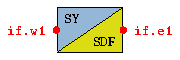
\includegraphics{figs/example-node-interface}
\lstinputlisting[linerange={5-5}]{figs/example-node-interface.tex}
\caption{The \texttt{\char`\\trans} draw command. The function anchors are accessed with \texttt{[name]-f.[anchor]} and the port anchors are accessed with \texttt{[name].[anchor]}}
\end{figure}
\hspace{1pt}\bookmark{\char`\\interface\opt{[options]}\opt{(name)}\opt{<position>}\man{\{domain~left\}}\man{\{domain~right\}};}

\noindent This command draws an interface from one domain to another (e.g. a MoC interface). It can be customized with the following keys (check \ref{sec:helper-options} for composite options):

\begin{optionslist}
\item \texttt{anchor=[anchor]} center point for shape. Default is \texttt{center}.
\item \texttt{xshift=[distance]} shift position in X direction. Default is \texttt{0pt}.
\item \texttt{yshift=[distance]} shift position in Y direction. Default is \texttt{0pt}.
\item \texttt{rotate=[number]} the rotation angle (in degrees) of the node. Default is \texttt{0}.
\end{optionslist}


\begin{figure}[htb]\centering
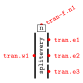
\includegraphics{figs/example-node-trans}
\lstinputlisting[linerange={5-5}]{figs/example-node-trans.tex}
\caption{The \texttt{\char`\\trans} draw command. The function anchors are accessed with \texttt{[name]-f.[anchor]} and the port anchors are accessed with \texttt{[name].[anchor]}}
\end{figure}
\hspace{1pt}\bookmark{\char`\\trans\opt{[options]}\opt{(name)}\opt{<position>}\man{\{\}};}

\noindent This command draws a transversal node over a path (usually 90 degrees), which symbolizes a structural transition of the path's type (e.g. permutation). The label is ignored, but the brackets are necessary to mark the end of the arguments. It can be customized with the following keys (check \ref{sec:helper-options} for composite options):

\begin{optionslist}
\item \texttt{shape=} any \texttt{TikZ} style option for the node shape. Check section \ref{sec:provided-shapes} for a list of library-provided shapes. Default is \texttt{rectangle}.
\item \texttt{type=} the type / constructor of that particular ForSyDe block. It is shown as the main label, rotated at 90 degrees.
\item \texttt{npw=[0..10]} number of ports on the left side of the node, i.e. the number of left port anchors.
\item \texttt{ni=[0..10]} alias for \texttt{npw}, stands for ``number of inputs''.
\item \texttt{npe=[0..10]} number of ports on the right side of the node, i.e. the number of right port anchors.
\item \texttt{no=[0..10]} alias for \texttt{npe}, stands for ``number of outputs''.
\item \texttt{nf=[0..4]} the number of passed functions. Default is \texttt{0}.
\item \texttt{f1=} first function label. Appears as a box in the upper part in case \texttt{nf > 0}. Default is $f_1$.
\item \texttt{f2=} second function label. Appears as a box in the upper part in case \texttt{nf > 1}. Default is $f_2$.
\item \texttt{f3=} third function label. Appears as a box in the upper part in case \texttt{nf > 2}. Default is $f_3$.
\item \texttt{f4=} fourth function label. Appears as a box in the upper part in case \texttt{nf > 3}. Default is $f_4$.
\item \texttt{anchor=[anchor]} center point for shape. Default is \texttt{center}.
\item \texttt{xshift=[distance]} shift position in X direction. Default is \texttt{0pt}.
\item \texttt{yshift=[distance]} shift position in Y direction. Default is \texttt{0pt}.
\item \texttt{rotate=[number]} the rotation angle (in degrees) of the node. Default is \texttt{0}.
\item \texttt{rotate shape=[number]} the rotation angle (in degrees) of the \texttt{shape}. Defailt is \texttt{0}.
\item \texttt{inner ysep=[distance]} the distance between the function node, the label node and the type node. Default is \texttt{3pt}.
\end{optionslist}

\begin{figure}[htb]\centering
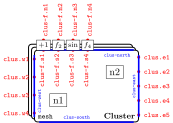
\includegraphics{figs/example-node-cluster}
\lstinputlisting[linerange={5-7}]{figs/example-node-cluster.tex}
\caption{The \texttt{\char`\\cluster} draw command. The function anchors are accessed with \texttt{[name]-f.[anchor]}, the port anchors are accessed with \texttt{[name].[anchor]} and the cluster outer shape edges are named \texttt{[name]-[position]}}
\end{figure}
\hspace{1pt}\bookmark{\char`\\cluster\opt{[options]}\opt{(name)}\man{<list~of~clustered~nodes>}\man{\{label\}};}

\noindent This command draws a cluster around other nodes. Instead of a position, it requires a list of nodes to fit. Apart from the functions and port anchors as seen in the previous commands, this command provides the edges of the outer shape cluster as names. These names can be used further in computing intersection points. It can be customized with the following keys (check \ref{sec:helper-options} for composite options):

\begin{optionslist}
\item \texttt{class=[sy|de|ct|sdf|blackbox|none]} The class of the node. This option affects the field color and the constructor label. Default is \texttt{none}.
\item \texttt{hasmoc} flag for saying that this node is a process, therefore it is associated with a MoC. It need to be provided otherwise the global flags will ignore MoC-related options (e.g. \texttt{nomoccolor}).
\item \texttt{shape=} any \texttt{TikZ} style option for the node shape. Check section \ref{sec:provided-shapes} for a list of library-provided shapes. Default is \texttt{rectangle}.
\item \texttt{type=} the type / constructor of that particular ForSyDe block. It shows below the main label and it is affected by the \texttt{class} argument.
\item \texttt{npw=[0..10]} number of ports on the left side of the node, i.e. the number of left port anchors.
\item \texttt{ni=[0..10]} alias for \texttt{npw}, stands for ``number of inputs''.
\item \texttt{npe=[0..10]} number of ports on the right side of the node, i.e. the number of right port anchors.
\item \texttt{no=[0..10]} alias for \texttt{npe}, stands for ``number of outputs''.
\item \texttt{nf=[0..4]} the number of passed functions. Default is \texttt{0}.
\item \texttt{f1=} first function label. Appears as a box in the upper part in case \texttt{nf > 0}. Default is $f_1$.
\item \texttt{f2=} second function label. Appears as a box in the upper part in case \texttt{nf > 1}. Default is $f_2$.
\item \texttt{f3=} third function label. Appears as a box in the upper part in case \texttt{nf > 2}. Default is $f_3$.
\item \texttt{f4=} fourth function label. Appears as a box in the upper part in case \texttt{nf > 3}. Default is $f_4$.
\item \texttt{anchor=[anchor]} center point for shape. Default is \texttt{center}.
\item \texttt{xshift=[distance]} shift position in X direction. Default is \texttt{0pt}.
\item \texttt{yshift=[distance]} shift position in Y direction. Default is \texttt{0pt}.
\item \texttt{rotate=[number]} the rotation angle (in degrees) of the node. Default is \texttt{0}.
\item \texttt{rotate shape=[number]} the rotation angle (in degrees) of the \texttt{shape}. Defailt is \texttt{0}.
\item \texttt{inner xsep=[distance]} the inner separation in X direction. Default is \texttt{3pt}.
\item \texttt{inner ysep=[distance]} the inner separation in Y direction. Default is \texttt{3pt}.
\end{optionslist}


% \begin{figure}[htb]\centering
% \includegraphics{figs/example-node-embed}
% \lstinputlisting[linerange={5-7}]{figs/example-node-embed.tex}
% \caption{The \texttt{\char`\\embed} draw command. It is basically \texttt{\char`\\cluster} but where the clustered nodes are passed as a parameter}
% \end{figure}
% \hspace{1pt}\bookmark{\char`\\embed\opt{[cluster~options]}\opt{(name)}\man{\{code~for~clustered~nodes\}};}

% \noindent This command is basically the same as \texttt{\char`\\cluster} but it takes the code for the clustered nodes as a parameter.


\begin{figure}[htb]\centering
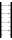
\includegraphics{figs/example-node-drawconduit}
\lstinputlisting[linerange={5-8}]{figs/example-node-drawconduit.tex}
\caption{The \texttt{\char`\\drawconduit} draw command.}
\end{figure}
\hspace{1pt}\bookmark{\char`\\drawconduit\opt[length]\man\{node~with~ports\}\{num.~ports~west\}\{num.~ports~east\};}

\noindent This command draws short lines outside a node with port anchors, that might be interpreted as ``conduits'' or ``ports''. It is used as helper for drawing, for example, custom-shaped transition patterns, like in the figure above.

\subsubsection{Shapes}
\label{sec:provided-shapes}
\bookmark{node shapes}
\textsc{ForSyDe-TikZ} provides a collection of raw shapes either as \textsc{TikZ} styles or as low-level \textsc{PGF} drawings. They are often used as arguments for drawing commands. Below is a list with them and their usage:


\begin{longtable} { | p{3cm} | c | p{9cm} | }
  \toprule
  \textbf{Shape}  & \textbf{Drawing} & \textbf{Description} \\
  \midrule
  \texttt{atom shape}
  & \vspace{0pt} \begin{tikzpicture}[baseline] \node[atom shape] {}; \end{tikzpicture}
  & meant to be used with the \texttt{\char`\\basic} command, it is a good candidate for depicting ForSyDe atoms or other primitive blocks.
  \\
  \texttt{nary atom shape}
  & \vspace{0pt} \begin{tikzpicture}[baseline] \node[nary atom shape] {}; \end{tikzpicture}
  & similar to \texttt{atom shape}, but suggests an n-tuple of blocks.
  \\
  \texttt{leaf shape}
  & \vspace{0pt} \begin{tikzpicture}[baseline] \node[leaf shape, inner sep=7pt] {}; \end{tikzpicture}
  &  meant to be used with the \texttt{\char`\\standard} command, it is a good candidate for depicting abstractions of complex semantics (e.g. black boxes).
  \\
  \texttt{nary leaf shape}
  & \vspace{0pt} \begin{tikzpicture}[baseline] \node[nary leaf shape, inner sep=7pt] {}; \end{tikzpicture}
  & similar to \texttt{leaf shape}, but suggests an n-tuple of blocks.
  \\
  \texttt{comp shape}
  & \vspace{0pt} \begin{tikzpicture}[baseline] \node[comp shape, inner sep=7pt] {}; \end{tikzpicture}
  &  meant to be used with the \texttt{\char`\\cluster} command, it is a good candidate for depicting exposed hierarchical blocks such as composite processes.
  \\
  \texttt{nary comp shape}
  & \vspace{0pt} \begin{tikzpicture}[baseline] \node[nary comp shape, inner sep=7pt] {}; \end{tikzpicture}
  & similar to \texttt{leaf shape}, but suggests an n-tuple of blocks.
  \\
  \texttt{\texttt{ports e[0..10]w[0..10]}}
  & \vspace{0pt} \begin{tikzpicture}[baseline] \node[ports e1w1] {}; \end{tikzpicture}
  & these are multiple shapes that have no drawing, but define additional anchors\footnote{apart from the ones inherited from \texttt{rectangle}} for ports on the east (\texttt{.e[index]}) and west (\texttt{.w[index]}) sides of the node. It is meant to fit around an existing shape. 
  \\
  \texttt{\texttt{func[0..4]}}
  & \vspace{0pt} \begin{tikzpicture}[baseline] \node[func4] {\functionlabels{4}{a}{b}{c}{d}}; \end{tikzpicture}
  & these shapes create a series of boxes with text and for each box two anchors: north (\texttt{.n[index]}), south (\texttt{.s[index]}). They are used to show functions as input arguments.
  \\
  \texttt{\texttt{dp shape}}
  & \vspace{0pt} \begin{tikzpicture}[baseline] \node[dp shape, inner sep=7pt] {}; \end{tikzpicture}
  & meant to be used with the \texttt{\char`\\cluster} command, this shape suggests a data parallel skeleton.
  \\
  \texttt{\texttt{pipe shape}}
  & \vspace{0pt} \begin{tikzpicture}[baseline] \node[pipe shape, inner sep=7pt] {}; \end{tikzpicture}
  & meant to be used with the \texttt{\char`\\cluster} command, this shape suggests a pipeline skeleton.
  \\
  \texttt{\texttt{merge shape}}
  & \vspace{0pt} \begin{tikzpicture}[baseline] \node[merge shape, inner sep=7pt] {}; \end{tikzpicture}
  & meant to be used with the \texttt{\char`\\cluster} command, this shape suggests a reduce/recur skeleton.
  \\
  \texttt{\texttt{generic skel shape}}
  & \vspace{0pt}\begin{tikzpicture}[baseline] \node[generic skel shape, inner sep=7pt] {}; \end{tikzpicture}
  & meant to be used with the \texttt{\char`\\cluster} command, this shape suggests generic skeleton which implies a recursive composition of functions/blocks.
  \\
  \texttt{\texttt{trans shape v[1..8]v[1..8]}}
  & \vspace{0pt}\begin{tikzpicture}[baseline] \node[trans shape v2v3, inner ysep=10pt] {}; \end{tikzpicture}
  & meant to be used with the \texttt{\char`\\trans} command, this shape suggests a transition in the structure of \texttt{n} input vectors resulting in \texttt{n'} output vectors.
  \\
  \texttt{\texttt{trans shape s1v1}}
  & \vspace{0pt}\begin{tikzpicture}[baseline] \node[trans shape s1v1, inner ysep=10pt] {}; \end{tikzpicture}
  & meant to be used with the \texttt{\char`\\trans} command, this shape suggests a transposition of a vector to/from a stream.
  \\
  \texttt{\texttt{trans shape v1gv1}}
  & \vspace{0pt}\begin{tikzpicture}[baseline] \node[trans shape v1gv1, inner ysep=10pt] {}; \end{tikzpicture}
  & meant to be used with the \texttt{\char`\\trans} command, this shape suggests a grouping/merging to/from a vector of vectors.
  \\
  \bottomrule
\end{longtable}

\subsubsection{Helper options}
\label{sec:helper-options}

\bookmark{node helper keys}
The \texttt{forsyde-tikz} library provides a large set of styles or function keys that can be used for user convenience as options in the draw commands shown in section \ref{sec:draw-commands}. 

\begin{longtable} { r|p{11cm} }
  \toprule
  \textbf{Key}  & \textbf{Description/Expands to}  \\
  \midrule
  \texttt{moc=x} & \texttt{hasmoc, class=x} \\
  \texttt{inner sep=x} & \texttt{inner xsep=x, inner ysep=x} \\
  \texttt{left of=x} & positions left of node \texttt{x}, with an edge-to-edge distance = 1cm \\
  \texttt{right of=x} & positions right of node \texttt{x}, with an edge-to-edge distance = 1cm \\
  \texttt{above of=x} & positions above of node \texttt{x}, with an edge-to-edge distance = 1cm \\
  \texttt{below of=x} & positions below of node \texttt{x}, with an edge-to-edge distance = 1cm \\
  \texttt{f=\{a;b;c;d\}} & parses a string of functions separated by \texttt{;} and sets \texttt{nf}, \texttt{f1}, \texttt{f2}, \texttt{f3} and \texttt{f4} accordingly \\
  \texttt{primitive} & \texttt{shape=atom shape} \\
  \texttt{primitiven} & \texttt{shape=nary atom shape} \\
  \texttt{process} & \texttt{shape=leaf shape, hasmoc} \\
  \texttt{processn} & \texttt{shape=nary leaf shape, hasmoc} \\
  \texttt{composite} & \texttt{shape=comp shape} \\
  \texttt{compositen} & \texttt{shape=comp shape} \\
  \texttt{embed} & \texttt{shape=leaf shape, hasmoc, inner sep=15pt} \\
  \texttt{farmstyle} & \texttt{shape=dp shape, inner xsep = 15pt, inner ysep = 20pt,} \\
  \texttt{pipestyle} & \texttt{shape=pipe shape, inner xsep = 15pt, inner ysep = 20pt,} \\
  \texttt{skeleton} & \texttt{shape=generic skel shape, inner xsep = 15pt, inner ysep = 20pt,} \\
  \texttt{transition=v2v3} & \texttt{shape=trans shape v2v3}. Default argument is \texttt{v1v1}. \\
  \texttt{zipx} & \texttt{transition={s1v1}, rotate shape=180, type=zipx,} \\
  \texttt{unzipx} & \texttt{transition={s1v1}, type=unzipx,} \\
  \bottomrule
\end{longtable}


\subsection{Paths}

Data flow in \texttt{forsyde-tikz} is represented as (directed) edges between components. These are regular \textsc{TikZ} paths, customized with a series of keys provided by the library. There are obvious advantages for using the \textsc{TikZ} infrastructure, such as being able to further customize paths outside the scope of this library, or reuse existing keys (e.g. the arrow tips, shapes). The custom port or function anchors presented in the previous section come in handy when considering port-to-port connections. 


\begin{figure}[htb]\centering
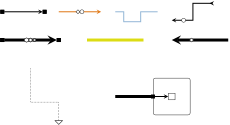
\includegraphics{figs/example-paths}
\lstinputlisting[linerange={6-16}]{figs/example-paths.tex}
\caption{Different paths created with the library provided styles}
\end{figure}

The library provides the following custom keys:\bookmark{path keys}

\begin{optionslist}
\item \texttt{s=[MoC]} draws a signal. If the global options allow it, passing a MoC string to this key will color the signal accordingly. 
\item \texttt{sn=[MoC]} draws an n-tuple of signals. If the global options allow it, passing a MoC string to this key will color the signal accordingly. 
\item \texttt{v=[MoC]} draws a vector. If the global options allow it, passing a MoC string to this key will color the vector accordingly, suggesting that it contains signals of their respective MoC.
\item \texttt{vn=[MoC]} draws an n-tuple of vectors. If the global options allow it, passing a MoC string to this key will color the vector accordingly, suggesting that it contains signals of their respective MoC.
\item \texttt{f} draws an edge used for showing how functions and parameters are passed from higher order functions downwards into the hierarchy.  
\item \texttt{fn} similar to \texttt{f}, but for n-tuples of functions.  
\item \texttt{srcport} draws a port symbol at the source of the path.
\item \texttt{dstport} draws a port symbol at the destination of the path.
\item \texttt{token=[token-string]} draws symbols for depicting the data structures carried by ForSyDe signals or vectors. The accepted tokens strings are \texttt{scalar|vector|function}. To draw tuple structures you have to separate token keywords by \texttt{-} (dash). E.g.: 3-tuple of scalar,  vector and function can be drawn with \texttt{token=scalar-vector-function}. To depict functions which take other data types as arguments, you can group some tokens between parentheses. E.g. a 2-tuple of a scalar and a function which takes a vector and a scalar as arguments can be drawn with \texttt{token=scalar-(vector-scalar)}.
\item \texttt{token pos=[0.0 .. 1.0]} the position between the start node/anchor and the end node/anchor of the token symbols' center position. Default is \texttt{0.5}.
\item \texttt{intersect=[path-name]} finds the first intersection with the path named \texttt{[path-name]}, and creates a coordinate from it, named by default \texttt{int} if no other name was given with the \texttt{as} key.
\item \texttt{as=[coordinate-name]} names the intersection coordinate found with the \texttt{intersect}.
\item \texttt{trans=\{source-path-style\}\{intersection-path-name\}\{destination-path-style\}} is a helper key which finds the intersection of the current path with \texttt{intersection-path-name}, splits the current path into two, decorated with \texttt{source-path-style} and  \texttt{destination-path-style} respectively.
\item \texttt{-|-=[0.0 .. 1.0]} will create a horizontal-vertical-horizontal spline in the path. It may be accompanied by a number which determines the position of the 90 degree angle.
\item \texttt{|-|=[0.0 .. 1.0]} will create a vertical-horizontal-vertical spline in the path. It may be accompanied by a number which determines the position of the 90 degree angle.
\item \texttt{-|-=[0.0 .. 1.0]} will create a horizontal-vertical-horizontal spline in the path. It may be accompanied by a number which determines the position of the 90 degree angle.
\item \texttt{-|-|=[0.0 .. 1.0]} will create a horizontal-vertical-horizontal-vertical spline in the path. It may be accompanied by a number which determines the position of the 90 degree angle.
\item \texttt{-|-|-=[0.0 .. 1.0]:[0.0 .. 1.0]} will create a horizontal-vertical-horizontal-vertical-horizontal spline in the path. It may be accompanied by two numbers  separated by \texttt{:} which determine the position of the 90 degree angles.
\item \texttt{|-|-|=[0.0 .. 1.0]:[0.0 .. 1.0]} will create a vertical-horizontal-vertical-horizontal-vertical spline in the path. It may be accompanied by two numbers  separated by \texttt{:} which determine the position of the 90 degree angles.
\item \texttt{deviate=} is a length representing the deviation from the straight path in case of complex splines (\texttt{-|-|},\texttt{-|-|-} and \texttt{|-|-|}).
\end{optionslist}

\subsubsection{Helper commands}
\label{sec:helper-commands}

The following commands can be alternatively used to draw paths, in case the complexity of the \texttt{\string\path} \textsc{TikZ} command is not needed. The MoC can be passed to the \texttt{moc} style key.\\

\hspace{1pt}\bookmark{\texttt{\string\signal\man[style]~\man(from)~arrow-tip~(to)};}

\hspace{1pt}\bookmark{\texttt{\string\signaln\man[style]~\man(from)~arrow-tip~(to)};}

\hspace{1pt}\bookmark{\texttt{\string\vector\man[style]~\man(from)~arrow-tip~(to)};}

\hspace{1pt}\bookmark{\texttt{\string\vectorn\man[style]~\man(from)~arrow-tip~(to)};}

\hspace{1pt}\bookmark{\texttt{\string\function\man[style]~\man(from)~arrow-tip~(to)};}

\hspace{1pt}\bookmark{\texttt{\string\functionn\man[style]~\man(from)~arrow-tip~(to)};}\\\\

\subsection{Utility commands}

Following is a list of miscellaneous functions and environments provided for user convenience:\\

\hspace{1pt}\bookmark{\texttt{\string\textleftof\{node\}\{text\}}}

\hspace{1pt}\bookmark{\texttt{\string\textrightof\{node\}\{text\}}}

\hspace{1pt}\bookmark{\texttt{\string\textaboveof\{node\}\{text\}}}

\hspace{1pt}\bookmark{\texttt{\string\textbelowof\{node\}\{text\}}}

\hspace{1pt}\bookmark{\texttt{\string\ifnodedefined\{node\}\{true~expr\}\{false~expr\}}}\\

\noindent Conditional sub-drawing if a node has been defined or not. Useful for ignoring edge cases when drawing recursive structures with \texttt{\string\foreach}.

\hspace{1pt}\bookmark{\char`\\gettikzx\man\{node\}\{\char`\\xmacro\}}

\noindent Gets the \texttt{X} coordinate of \texttt{node} and stores it in \texttt{\string\xmacro}.

\hspace{1pt}\bookmark{\char`\\gettikzy\man\{node\}\{\char`\\ymacro\}}

\noindent Gets the \texttt{Y} coordinate of \texttt{node} and stores it in \texttt{\string\ymacro}.

\hspace{1pt}\bookmark{\char`\\gettikzxy\man\{node\}\{\char`\\xmacro\}\{\char`\\ymacro\}}

\noindent Gets the \texttt{X} and \texttt{Y} coordinates of \texttt{node} and stores them in \texttt{\string\xmacro} and  \texttt{\string\ymacro} respectively.

\begin{figure}[htb]\centering
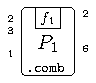
\includegraphics{figs/example-utility-portinfo}
\lstinputlisting[linerange={5-6}]{figs/example-utility-portinfo.tex}
\caption{An example of using the \texttt{\string\resetportinfo}, \texttt{\string\epinfo} and \texttt{\string\wpinfo} commands}
\end{figure}
\hspace{1pt}\bookmark{\char`\\resetportinfo\man\{node\}}

\noindent Resets the counters for the \texttt{\string\epinfo} and \texttt{\string\wpinfo} commands which decorates ports with information. These commands can be used for decorating ports, for example, with production and consumption rates in case of SDF processes.

\hspace{1pt}\bookmark{\char`\\wpinfo\opt[anchor]\man\{label\}}

\noindent Places a label node next to a western port and increases its counter.

\hspace{1pt}\bookmark{\char`\\epinfo\opt[anchor]\man\{label\}}

\noindent Places a label node next to a eastern port and increases its counter.

\subsection{Further customizing the environment}

The following commands can be used in the document preamble for changing environment variables.
\begin{lstlisting}
% Colors
\renewcommand{\defaultdrawcolor}{[color]}
\renewcommand{\defaultfillcolor}{[color]}
\definecolor{sycolor}{[coord sys]}{[color coord]}
\definecolor{ctcolor}{[coord sys]}{[color coord]}
\definecolor{decolor}{[coord sys]}{[color coord]}
\definecolor{sdfcolor}{[coord sys]}{[color coord]}
\definecolor{blackboxcolor}{[coord sys]}{[color coord]}}
% line widths
\renewcommand{\compositelinewidth}{[size]}
\renewcommand{\skeletonlinewidth}{[size]} 
\renewcommand{\signalpathlinewidth}{[size]}
\renewcommand{\functionpathlinewidth}{[size]}
\renewcommand{\vectorpathlinewidth}{[size]}
% sizes, etc.
\renewcommand{\tokensize}{[size]}
\renewcommand{\halftokensize}{[size]}
\end{lstlisting}


%%% Local Variables:
%%% TeX-command-default: "Make"
%%% mode: latex
%%% TeX-master: "../refman"
%%% End:
